\documentclass[11pt,a4paper]{article}

% -----------------------------------------------------------------------------
% PACKAGES & TYPOGRAPHY
% -----------------------------------------------------------------------------
\usepackage[utf8]{inputenc}
\usepackage[T1]{fontenc}
\usepackage{lmodern}
\usepackage[margin=0.85in,headheight=14pt]{geometry}
\usepackage{amsmath,amssymb}
\usepackage{booktabs}
\usepackage{tabularx}
\usepackage{multirow}
\usepackage{array}
\usepackage{listings}
\usepackage{xcolor}
\usepackage{graphicx}
\graphicspath{{images/}}
\usepackage{tikz}
\usetikzlibrary{arrows.meta, positioning, shapes.geometric, calc}
\usepackage{fancyhdr}
\usepackage{titlesec}
\usepackage{caption}
\usepackage{microtype}
\usepackage{hyperref}

% -----------------------------------------------------------------------------
% COLOR SCHEME
% -----------------------------------------------------------------------------
\definecolor{primaryblue}{RGB}{24, 43, 73}
\definecolor{secondaryblue}{RGB}{41, 128, 185}
\definecolor{accentgray}{RGB}{245, 247, 250}
\definecolor{darkgray}{RGB}{60, 64, 67}
\definecolor{bordergray}{RGB}{218, 224, 233}
\definecolor{vgreen}{RGB}{39, 140, 56}
\definecolor{vpurple}{RGB}{125, 40, 140}

% -----------------------------------------------------------------------------
% HYPERLINK SETUP (NO EXTERNAL CITATIONS)
% -----------------------------------------------------------------------------
\hypersetup{
    colorlinks=true,
    linkcolor=primaryblue,
    urlcolor=secondaryblue,
    pdfauthor={Jayakody J.A.K., Attanayake A.Y., Rajinthan R.},
    pdftitle={EN4021 ADS: Multi-Master System Bus Design Report}
}

% -----------------------------------------------------------------------------
% HEADERS & FOOTERS
% -----------------------------------------------------------------------------
\pagestyle{fancy}
\fancyhf{}
\fancyhead[L]{\small\color{darkgray}EN4021: System Bus Design Report}
\fancyhead[R]{\small\color{darkgray}\thepage}
\renewcommand{\headrulewidth}{0.4pt}
\renewcommand{\footrulewidth}{0pt}

% -----------------------------------------------------------------------------
% SECTION STYLES
% -----------------------------------------------------------------------------
\titleformat{\section}
  {\color{primaryblue}\normalfont\Large\bfseries}{\thesection}{1em}{}[{\titlerule[0.8pt]}]
\titleformat{\subsection}
  {\color{secondaryblue}\normalfont\large\bfseries}{\thesubsection}{1em}{}
\titleformat{\subsubsection}
  {\color{primaryblue}\normalfont\normalsize\bfseries}{\thesubsubsection}{1em}{}

% -----------------------------------------------------------------------------
% VERILOG LISTINGS STYLE
% -----------------------------------------------------------------------------
\lstdefinestyle{cleanverilog}{
    language=Verilog,
    basicstyle=\ttfamily\scriptsize\color{black},
    keywordstyle=\color{primaryblue}\bfseries,
    commentstyle=\color{vgreen}\itshape,
    stringstyle=\color{vpurple},
    numbers=left,
    numberstyle=\tiny\color{darkgray},
    stepnumber=1,
    numbersep=8pt,
    backgroundcolor=\color{accentgray},
    showspaces=false,
    showstringspaces=false,
    showtabs=false,
    frame=single,
    rulecolor=\color{bordergray},
    tabsize=2,
    captionpos=b,
    breaklines=true,
    breakatwhitespace=false
}
\lstset{style=cleanverilog}

% -----------------------------------------------------------------------------
% DOCUMENT
% -----------------------------------------------------------------------------
\begin{document}

% -----------------------------------------------------------------------------
% COVER PAGE
% -----------------------------------------------------------------------------
\begin{titlepage}
    \centering
    \vspace*{0.5cm}
    {\scshape\LARGE Department of Electronic and Telecommunication Engineering \par}
    \vspace{0.3cm}
    {\scshape\Large University of Moratuwa, Sri Lanka \par}
    \vspace{1.2cm}
    
    
\begin{tikzpicture}
        \draw[primaryblue, line width=2pt] (-7,0) -- (7,0);
    \end{tikzpicture}
    \vspace{0.3cm}
    
    {\huge\bfseries\color{primaryblue} EN4021: Advanced Digital Systems \par}
    \vspace{0.3cm}
    {\Large\bfseries Shared On-Chip Bus Interconnect Architecture with Split-Transaction Protocol and Cross-FPGA UART Bridge Verification \par}
    \vspace{0.3cm}
    
    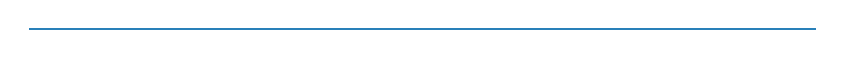
\begin{tikzpicture}
        \draw[secondaryblue, line width=1pt] (-5,0) -- (5,0);
    \end{tikzpicture}
    
    \vspace{1.5cm}

    \begin{minipage}[t]{0.50\textwidth}
        \flushleft
        \textbf{Student Team:}\\
        \vspace{0.2cm}
        \textbf{Jayakody J.A.K.} --- \texttt{220247J}\\
        \textbf{Attanayake A.Y.} --- \texttt{220051D}\\
        \textbf{Rajinthan R.} --- \texttt{220502M}
    \end{minipage}
    \hfill
    \begin{minipage}[t]{0.46\textwidth}
        \flushright
        \textbf{Target Hardware:}\\
        \vspace{0.2cm}
        \textbf{Board 1:} DE0-Nano (\texttt{EP4CE22F17C6N})\\
        \textbf{Board 2:} DE2-115 (\texttt{EP4CE115F29C7N})\\
        \textbf{System Clock:} 50~MHz Synchronous\\
        \textbf{Toolchain:} Quartus Prime / ModelSim
    \end{minipage}

    \vspace{2.0cm}
    
    \begin{minipage}[c]{0.95\textwidth}
        \centering
        \small\textbf{Abstract}\\
        This report details the RTL design, synthesis, and hardware verification of a 14-bit address, 8-bit data shared synchronous bus. The system includes two initiator masters and four targets, using fixed-priority arbitration with a hardware split-transaction mechanism on multi-cycle reads to eliminate head-of-line blocking. Inter-board transactions are routed through an active 9600-baud serial bridge between an Altera DE0-Nano and a DE2-115. Real-time verification was performed on-chip using JTAG In-System Sources and Probes (ISSP).
    \end{minipage}

    \vfill
    {\large\bfseries Technical Course Project Report \par}
    \vspace{0.2cm}
    {\normalsize September 2026 \par}
\end{titlepage}

\newpage
\tableofcontents
\newpage

% -----------------------------------------------------------------------------
% SECTION 1: ARCHITECTURAL OVERVIEW
% -----------------------------------------------------------------------------
\section{System Architecture and Overview}

We implemented a shared-bus interconnect running synchronously on a 50~MHz clock (\texttt{clk}) with an active-low asynchronous reset (\texttt{rst\_n}). The interface provides a 14-bit address bus (\texttt{bus\_addr[13:0]}), separate 8-bit write and read data buses (\texttt{bus\_wdata[7:0]}, \texttt{bus\_rdata[7:0]}), write control strobes, and ready handshakes.

\begin{figure}[h!]
\centering
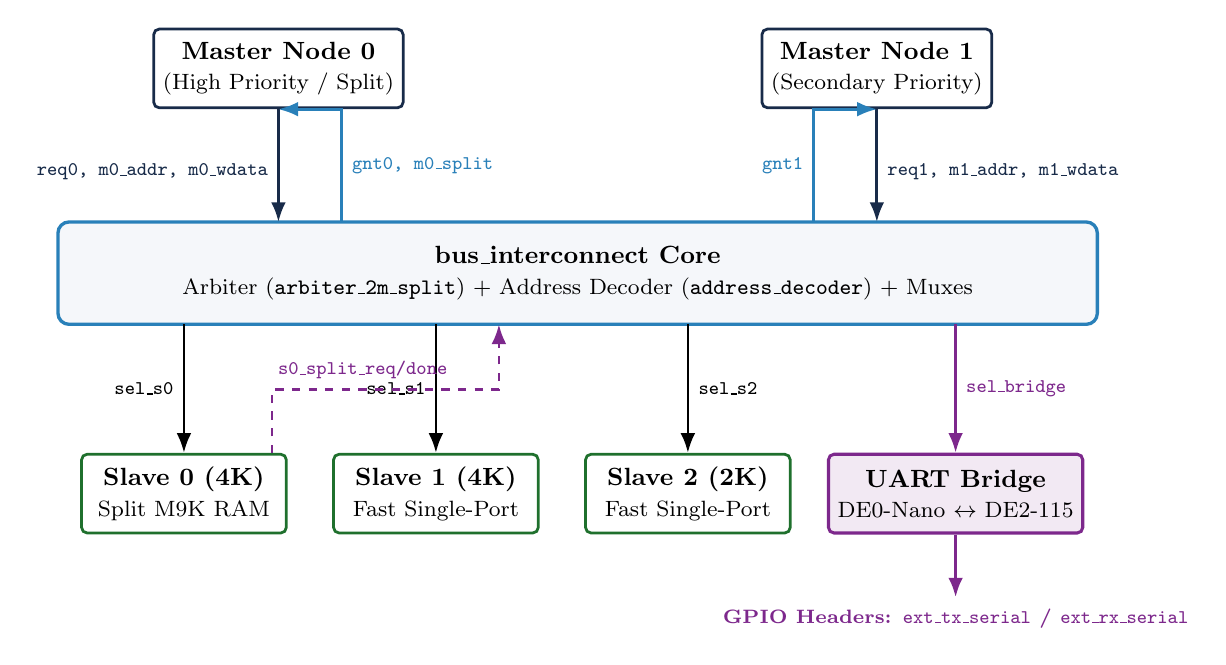
\begin{tikzpicture}[
    box/.style={draw=primaryblue, line width=1pt, fill=white, minimum width=2.7cm, minimum height=1.0cm, align=center, font=\small\bfseries, rounded corners=2pt},
    intercon/.style={draw=secondaryblue, line width=1.2pt, fill=accentgray, minimum width=13.2cm, minimum height=1.3cm, align=center, font=\small\bfseries, rounded corners=4pt},
    slave/.style={draw=vgreen!80!black, line width=1pt, fill=white, minimum width=2.6cm, minimum height=1.0cm, align=center, font=\small\bfseries, rounded corners=2pt},
    bridge/.style={draw=vpurple, line width=1.1pt, fill=vpurple!10, minimum width=2.8cm, minimum height=1.0cm, align=center, font=\small\bfseries, rounded corners=2pt},
    arr/.style={-{Latex[length=2.5mm]}, line width=1pt}
]
    % Masters
    \node[box] (m0) at (-3.8, 3.2) {Master Node 0\\ \footnotesize\textnormal{(High Priority / Split)}};
    \node[box] (m1) at (3.8, 3.2) {Master Node 1\\ \footnotesize\textnormal{(Secondary Priority)}};

    % Central Bus Interconnect
    \node[intercon] (bus) at (0, 0.6) {bus\_interconnect Core\\ \footnotesize\textnormal{Arbiter (\texttt{arbiter\_2m\_split}) + Address Decoder (\texttt{address\_decoder}) + Muxes}};

    % Slaves
    \node[slave] (s0) at (-5.0, -2.2) {Slave 0 (4K)\\ \footnotesize\textnormal{Split M9K RAM}};
    \node[slave] (s1) at (-1.8, -2.2) {Slave 1 (4K)\\ \footnotesize\textnormal{Fast Single-Port}};
    \node[slave] (s2) at (1.4, -2.2) {Slave 2 (2K)\\ \footnotesize\textnormal{Fast Single-Port}};
    \node[bridge] (bb) at (4.8, -2.2) {UART Bridge\\ \footnotesize\textnormal{DE0-Nano $\leftrightarrow$ DE2-115}};

    % Master Routing
    \draw[arr, color=primaryblue] (m0.south) -- ++(0,-0.8) -| (-3.8, 1.25) node[midway, left, font=\scriptsize] {\texttt{req0, m0\_addr, m0\_wdata}};
    \draw[arr, color=secondaryblue] (-3.0, 1.25) |- (m0.south) node[pos=0.25, right, font=\scriptsize] {\texttt{gnt0, m0\_split}};

    \draw[arr, color=primaryblue] (m1.south) -- ++(0,-0.8) -| (3.8, 1.25) node[midway, right, font=\scriptsize] {\texttt{req1, m1\_addr, m1\_wdata}};
    \draw[arr, color=secondaryblue] (3.0, 1.25) |- (m1.south) node[pos=0.25, left, font=\scriptsize] {\texttt{gnt1}};

    % Bus-to-Slave Routing
    \draw[arr] (-5.0, -0.05) -- (s0.north) node[midway, left, font=\scriptsize] {\texttt{sel\_s0}};
    \draw[arr] (-1.8, -0.05) -- (s1.north) node[midway, left, font=\scriptsize] {\texttt{sel\_s1}};
    \draw[arr] (1.4, -0.05) -- (s2.north) node[midway, right, font=\scriptsize] {\texttt{sel\_s2}};
    \draw[arr, color=vpurple] (4.8, -0.05) -- (bb.north) node[midway, right, font=\scriptsize] {\texttt{sel\_bridge}};

    % Split handshake
    \draw[arr, dashed, color=vpurple] (s0.north east) ++(-0.2,0) -- ++(0,0.8) -| node[pos=0.2, above, font=\scriptsize] {\texttt{s0\_split\_req/done}} (-1.0, -0.05);

    % Physical serial lines
    \draw[arr, color=vpurple, line width=1.3pt] (bb.south) -- ++(0,-0.8) node[below, font=\scriptsize\bfseries] {GPIO Headers: \texttt{ext\_tx\_serial} / \texttt{ext\_rx\_serial}};
\end{tikzpicture}
\caption{System block diagram showing masters, central interconnect, and target slaves.}
\label{fig:overall_arch}
\end{figure}

The interconnect prevents slow memory accesses from blocking high-speed transfers using hardware split transactions. When Master 0 initiates a read on the multi-cycle Slave 0, the slave drops its ready line and pulses a split-request signal. This causes the arbiter to revoke bus grant from Master 0 and reassign it to Master 1 for independent access. Once Slave 0 finishes fetching data from its internal RAM, it asserts a completion signal, prompting the arbiter to return bus ownership to Master 0 to latch the result.

An active UART bridge connects the local memory bus on the DE0-Nano board to a secondary DE2-115 board via 3.3V GPIO pins.

% -----------------------------------------------------------------------------
% SECTION 2: ADDRESS ALLOCATION
% -----------------------------------------------------------------------------
\section{Address Allocation and Memory Mapping}

The bus uses a 14-bit address bus addressing up to 16~KB of memory space. Table~\ref{tab:memory_allocation} lists the complete memory map.

\begin{table}[h!]
\centering
\caption{System Memory Map}
\label{tab:memory_allocation}
\small
\begin{tabularx}{\textwidth}{lllcX}
\toprule
\textbf{Target} & \textbf{Address Range} & \textbf{Bits [13:11]} & \textbf{Size} & \textbf{Access Type} \\
\midrule
\textbf{Slave 0} & \texttt{0x0000 -- 0x0FFF} & \texttt{000} or \texttt{001} & 4~KB & Single-cycle writes; 3-cycle split reads. \\
\textbf{Slave 1} & \texttt{0x1000 -- 0x1FFF} & \texttt{010} or \texttt{011} & 4~KB & Single-cycle read/write via M9K RAM. \\
\textbf{Slave 2} & \texttt{0x2000 -- 0x27FF} & \texttt{100} & 2~KB & Single-cycle read/write via M9K RAM. \\
\textbf{Unmapped Gap} & \texttt{0x2800 -- 0x2FFF} & \texttt{101} & 2~KB & Reserved hole; asserts \texttt{decode\_err}. \\
\textbf{UART Bridge} & \texttt{0x3000 -- 0x3FFF} & \texttt{110} or \texttt{111} & 4~KB & Cross-board serial packet link. \\
\bottomrule
\end{tabularx}
\end{table}

\subsection{Decoding Logic}
The combinational decoder evaluates the upper address bits as follows:
\begin{itemize}
    \item \textbf{Slave 0:} \texttt{addr[13:12] == 2'b00}
    \item \textbf{Slave 1:} \texttt{addr[13:12] == 2'b01}
    \item \textbf{Slave 2:} \texttt{addr[13:11] == 3'b100}
    \item \textbf{UART Bridge:} \texttt{addr[13:12] == 2'b11}
    \item \textbf{Decode Error:} Asserted when \texttt{bus\_valid} is high and \texttt{addr[13:11] == 3'b101}.
\end{itemize}

% -----------------------------------------------------------------------------
% SECTION 3: MODULE DESCRIPTORS
% -----------------------------------------------------------------------------
\section{Module Descriptions and Port Definitions}

This section details the interface and operational behavior of each sub-module in the design.

\subsection{Master Node (\texttt{master\_node})}
The master node accepts commands from a local interface, requests bus access from the arbiter, drives address and write data lines, and latches read data upon completion.

\begin{table}[h!]
\centering
\caption{Port List: \texttt{master\_node}}
\small
\begin{tabularx}{\textwidth}{lllcX}
\toprule
\textbf{Port} & \textbf{Width} & \textbf{Direction} & \textbf{Polarity} & \textbf{Description} \\
\midrule
\texttt{clk}, \texttt{rst\_n} & 1, 1 & Input & System & 50~MHz clock and active-low asynchronous reset. \\
\texttt{cmd\_start} & 1 & Input & Active-High & 1-cycle strobe to initiate a transfer. \\
\texttt{cmd\_we} & 1 & Input & Level & Write enable: 1 = write, 0 = read. \\
\texttt{cmd\_addr} & 14 & Input & Level & 14-bit target address. \\
\texttt{cmd\_wdata} & 8 & Input & Level & 8-bit write data payload. \\
\texttt{cmd\_rdata} & 8 & Output & Level & Latched read data returned to host. \\
\texttt{cmd\_done} & 1 & Output & Active-High & 1-cycle completion pulse returned to host. \\
\texttt{bus\_req} & 1 & Output & Active-High & Request output to arbiter. \\
\texttt{bus\_gnt} & 1 & Input & Active-High & Bus grant input from arbiter. \\
\texttt{bus\_split} & 1 & Input & Active-High & Notification from arbiter to suspend transaction. \\
\texttt{m\_addr} & 14 & Output & Level & Address driven to interconnect mux. \\
\texttt{m\_wdata} & 8 & Output & Level & Data driven to interconnect mux. \\
\texttt{m\_we} & 1 & Output & Level & Write enable driven to interconnect mux. \\
\texttt{m\_valid} & 1 & Output & Active-High & Indicates address and control lines are valid. \\
\texttt{bus\_rdata} & 8 & Input & Level & Read data return bus. \\
\texttt{bus\_ready} & 1 & Input & Active-High & Target ready handshake. \\
\bottomrule
\end{tabularx}
\end{table}

\begin{figure}[h!]
\centering
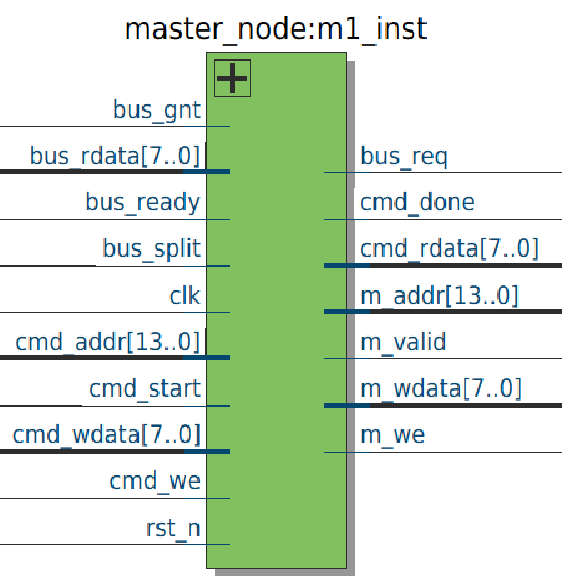
\includegraphics[width=0.52\textwidth]{Master.png}
\caption{RTL symbol of the plain master node (\texttt{master\_node}, instance \texttt{m1\_inst}) as elaborated by Quartus.}
\label{fig:rtl_master}
\end{figure}

\subsubsection{Master State Machine}
The master FSM operates across six states:
\begin{itemize}
    \item \texttt{IDLE (3'b000)}: Waits for \texttt{cmd\_start}. When asserted, latches command inputs, drives \texttt{bus\_req = 1}, and moves to \texttt{REQ}.
    \item \texttt{REQ (3'b001)}: Waits for \texttt{bus\_gnt}. Once granted, asserts \texttt{m\_valid = 1} and moves to \texttt{DRIVE}.
    \item \texttt{DRIVE (3'b010)}: If the slave asserts \texttt{bus\_split}, deasserts \texttt{m\_valid}, keeps \texttt{bus\_req = 1}, and moves to \texttt{SPLIT\_W}. If \texttt{bus\_ready} asserts, latches read data (on reads), asserts \texttt{cmd\_done}, and moves to \texttt{DONE}. If the slave remains busy, it moves to \texttt{WAIT}.
    \item \texttt{WAIT (3'b011)}: Waits for \texttt{bus\_ready} (moves to \texttt{DONE}) or \texttt{bus\_split} (moves to \texttt{SPLIT\_W}).
    \item \texttt{SPLIT\_W (3'b100)}: Holds \texttt{bus\_req = 1} while waiting for the split slave to finish. When re-granted (\texttt{bus\_gnt = 1}), asserts \texttt{m\_valid = 1} and returns to \texttt{DRIVE} to sample the prepared data.
    \item \texttt{DONE (3'b101)}: Clears all control flags and returns to \texttt{IDLE} on the next clock edge.
\end{itemize}

\subsection{Central Split Arbiter (\texttt{arbiter\_2m\_split})}
The arbiter prioritizes Master 0 over Master 1. If Master 0 encounters a split read on Slave 0, the arbiter temporarily grants the bus to Master 1. Once Slave 0 finishes data retrieval, Master 0 receives top priority to re-acquire the bus.

\begin{table}[h!]
\centering
\caption{Port List: \texttt{arbiter\_2m\_split}}
\small
\begin{tabularx}{\textwidth}{lllcX}
\toprule
\textbf{Port} & \textbf{Width} & \textbf{Direction} & \textbf{Polarity} & \textbf{Description} \\
\midrule
\texttt{clk}, \texttt{rst\_n} & 1, 1 & Input & System & Clock and reset lines. \\
\texttt{req0}, \texttt{req1} & 1, 1 & Input & Active-High & Request lines from Master 0 and Master 1. \\
\texttt{gnt0}, \texttt{gnt1} & 1, 1 & Output & Active-High & Grant outputs to Master 0 and Master 1. \\
\texttt{s0\_split\_req} & 1 & Input & Active-High & Split request strobe from Slave 0. \\
\texttt{s0\_split\_done} & 1 & Input & Active-High & Background ready strobe from Slave 0. \\
\texttt{m0\_split\_notify} & 1 & Output & Active-High & Split notice sent to Master 0. \\
\texttt{m1\_split\_notify} & 1 & Output & Active-High & Split notice sent to Master 1. \\
\bottomrule
\end{tabularx}
\end{table}

\subsection{Address Decoder (\texttt{address\_decoder})}
Combinational module that decodes the upper address bits whenever \texttt{bus\_valid} is high, generating one-hot select signals for the targets.

\begin{table}[h!]
\centering
\caption{Port List: \texttt{address\_decoder}}
\small
\begin{tabularx}{\textwidth}{lllcX}
\toprule
\textbf{Port} & \textbf{Width} & \textbf{Direction} & \textbf{Polarity} & \textbf{Description} \\
\midrule
\texttt{addr} & 14 & Input & Level & Active bus address. \\
\texttt{bus\_valid} & 1 & Input & Active-High & Transaction valid qualifier. \\
\texttt{sel\_s0} & 1 & Output & Active-High & Select line for Slave 0 (\texttt{0x0000 -- 0x0FFF}). \\
\texttt{sel\_s1} & 1 & Output & Active-High & Select line for Slave 1 (\texttt{0x1000 -- 0x1FFF}). \\
\texttt{sel\_s2} & 1 & Output & Active-High & Select line for Slave 2 (\texttt{0x2000 -- 0x27FF}). \\
\texttt{sel\_bridge} & 1 & Output & Active-High & Select line for UART bridge (\texttt{0x3000 -- 0x3FFF}). \\
\texttt{decode\_err} & 1 & Output & Active-High & Unmapped space flag (\texttt{0x2800 -- 0x2FFF}). \\
\bottomrule
\end{tabularx}
\end{table}

\subsection{Slave 0: 4~KB Split RAM (\texttt{slave\_0\_split\_4k})}
Slave 0 implements a 4~KB memory using an embedded Cyclone IV M9K block configured in simple dual-port mode. Port A executes single-cycle writes. Port B handles reads using a 3-cycle split-latency pipeline (\texttt{SPLIT\_LATENCY = 3}).

\begin{table}[h!]
\centering
\caption{Port List: \texttt{slave\_0\_split\_4k}}
\small
\begin{tabularx}{\textwidth}{lllcX}
\toprule
\textbf{Port} & \textbf{Width} & \textbf{Direction} & \textbf{Polarity} & \textbf{Description} \\
\midrule
\texttt{clk}, \texttt{rst\_n} & 1, 1 & Input & System & Clock and reset inputs. \\
\texttt{sel} & 1 & Input & Active-High & Target select line (\texttt{sel\_s0}). \\
\texttt{we} & 1 & Input & Level & Write enable: 1 = write, 0 = read. \\
\texttt{addr} & 12 & Input & Level & 12-bit word address within 4~KB range. \\
\texttt{din} & 8 & Input & Level & 8-bit bus write data. \\
\texttt{dout} & 8 & Output & Level & 8-bit bus read data. \\
\texttt{ready} & 1 & Output & Active-High & Transaction acknowledge handshake. \\
\texttt{split\_req} & 1 & Output & Active-High & Strobe sent to arbiter to request transaction split. \\
\texttt{split\_done} & 1 & Output & Active-High & Strobe sent to arbiter when data fetch finishes. \\
\bottomrule
\end{tabularx}
\end{table}

\begin{figure}[h!]
\centering
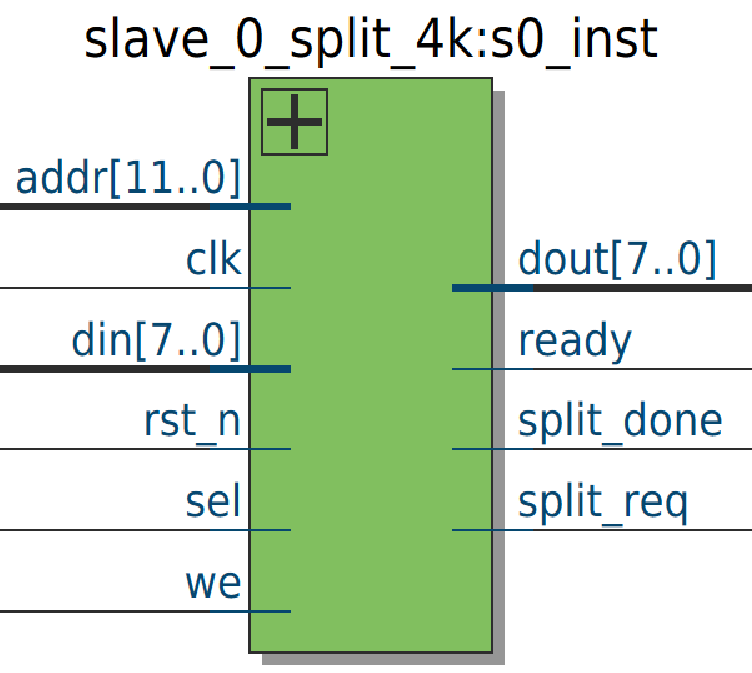
\includegraphics[width=0.50\textwidth]{Slave_4k.png}
\caption{RTL symbol of the 4~KB split slave (\texttt{slave\_0\_split\_4k}), showing the \texttt{split\_req}/\texttt{split\_done} handshake outputs that no other slave carries.}
\label{fig:rtl_slave0}
\end{figure}

\subsection{Slaves 1 and 2: Fast Single-Port RAM (\texttt{slave\_fast\_ram})}
Slaves 1 and 2 use single-port M9K blocks in \texttt{NEW\_DATA\_NO\_NBE\_READ} mode. Slave 1 uses a 12-bit address (4~KB), while Slave 2 uses an 11-bit address (2~KB). Handshakes are registered directly (\texttt{ready <= sel}), completing transactions in one cycle.

\begin{table}[h!]
\centering
\caption{Port List: \texttt{slave\_fast\_ram}}
\small
\begin{tabularx}{\textwidth}{lllcX}
\toprule
\textbf{Port} & \textbf{Width} & \textbf{Direction} & \textbf{Polarity} & \textbf{Description} \\
\midrule
\texttt{clk}, \texttt{rst\_n} & 1, 1 & Input & System & Clock and reset lines. \\
\texttt{sel} & 1 & Input & Active-High & Target select line (\texttt{sel\_s1} or \texttt{sel\_s2}). \\
\texttt{we} & 1 & Input & Level & Write enable. \\
\texttt{addr} & \texttt{AW} & Input & Level & Local address (12 bits for S1, 11 bits for S2). \\
\texttt{din} & 8 & Input & Level & 8-bit write data. \\
\texttt{dout} & 8 & Output & Level & 8-bit read data directly from M9K output register. \\
\texttt{ready} & 1 & Output & Active-High & 1-cycle handshake signal. \\
\bottomrule
\end{tabularx}
\end{table}

\begin{figure}[h!]
\centering
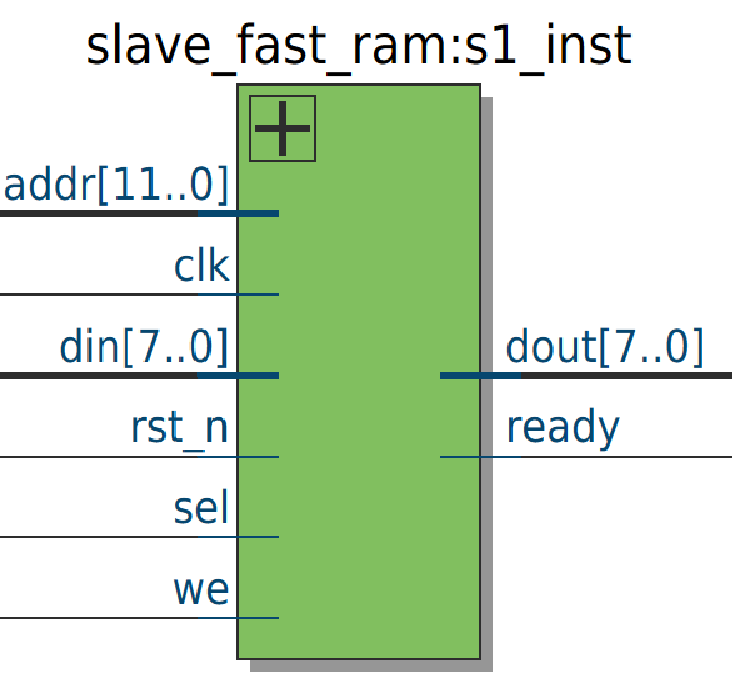
\includegraphics[width=0.50\textwidth]{Slave_2k.png}
\caption{RTL symbol of a fast single-port slave (\texttt{slave\_fast\_ram}, instance \texttt{s1\_inst}). Slave 2 is the same module with \texttt{AW = 11}.}
\label{fig:rtl_slavefast}
\end{figure}

\subsection{Cross-FPGA UART Bridge (\texttt{cross\_fpga\_bridge})}
The bridge bridges bus transactions across development boards. When an initiator accesses the range \texttt{0x3000 -- 0x3FFF}, the local Bridge Slave packs the 1-bit mode, 14-bit address, and 8-bit data into a 23-bit UART frame ($5208$ clock cycles per bit at 9600 baud, 50~MHz) transmitted over \texttt{ext\_tx\_serial}. The receiving Bridge Master on the DE2-115 deserializes the command, runs the local bus access, and returns the 8-bit read byte over \texttt{ext\_rx\_serial}.

\begin{table}[h!]
\centering
\caption{Port List: \texttt{cross\_fpga\_bridge}}
\small
\begin{tabularx}{\textwidth}{lllcX}
\toprule
\textbf{Port} & \textbf{Width} & \textbf{Direction} & \textbf{Polarity} & \textbf{Description} \\
\midrule
\texttt{clk}, \texttt{rst\_n} & 1, 1 & Input & System & 50~MHz clock and reset. \\
\texttt{sel} & 1 & Input & Active-High & Target select line (\texttt{sel\_bridge}). \\
\texttt{we} & 1 & Input & Level & Write enable. \\
\texttt{addr} & 12 & Input & Level & Offset address in bridge space. \\
\texttt{din} & 8 & Input & Level & Local master write data. \\
\texttt{dout} & 8 & Output & Level & Read data byte returned from remote FPGA. \\
\texttt{ready} & 1 & Output & Active-High & Acknowledge returned upon remote completion. \\
\texttt{ext\_rx\_serial} & 1 & Input & Serial & Physical UART RX pin (GPIO pin). \\
\texttt{ext\_tx\_serial} & 1 & Output & Serial & Physical UART TX pin (GPIO pin). \\
\bottomrule
\end{tabularx}
\end{table}

\begin{figure}[h!]
\centering
\includegraphics[width=0.50\textwidth]{{UART controlling master}}
\caption{RTL symbol of the UART-capable master (\texttt{master\_node\_uart}, instance \texttt{m0\_inst}) that carries the cross-FPGA link. Alongside the ordinary command and bus ports it exposes \texttt{cmd\_remote}, \texttt{cmd\_error} and the two serial pins.}
\label{fig:rtl_uart_master}
\end{figure}

\subsection{Top-Level Bus System (\texttt{top\_bus\_system})}
The module \texttt{top\_bus\_system} connects Master 0, Master 1, Slave 0, Slave 1, Slave 2, and the UART Bridge through the \texttt{bus\_interconnect} multiplexer logic. It exposes host command ports for both masters alongside physical serial pins for the external bridge.

\begin{figure}[h!]
\centering
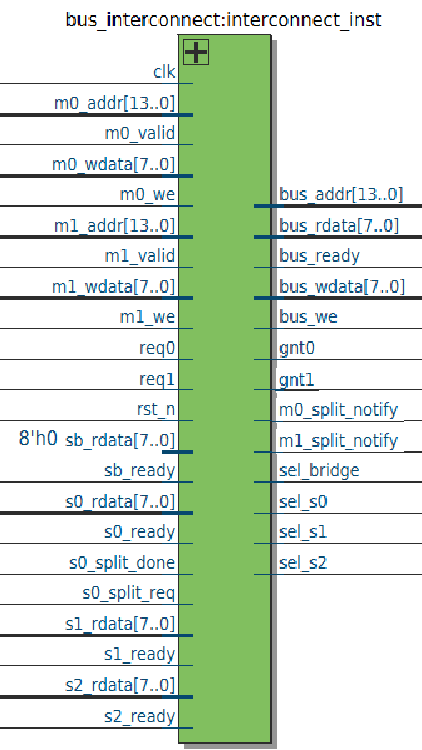
\includegraphics[width=0.42\textwidth]{Bus_Interconnect.png}
\caption{RTL symbol of \texttt{bus\_interconnect}: both master port groups and every slave return path enter on the left, and the shared bus, the grant lines, the split notifications and the one-hot selects leave on the right.}
\label{fig:rtl_interconnect}
\end{figure}

\begin{figure}[h!]
\centering
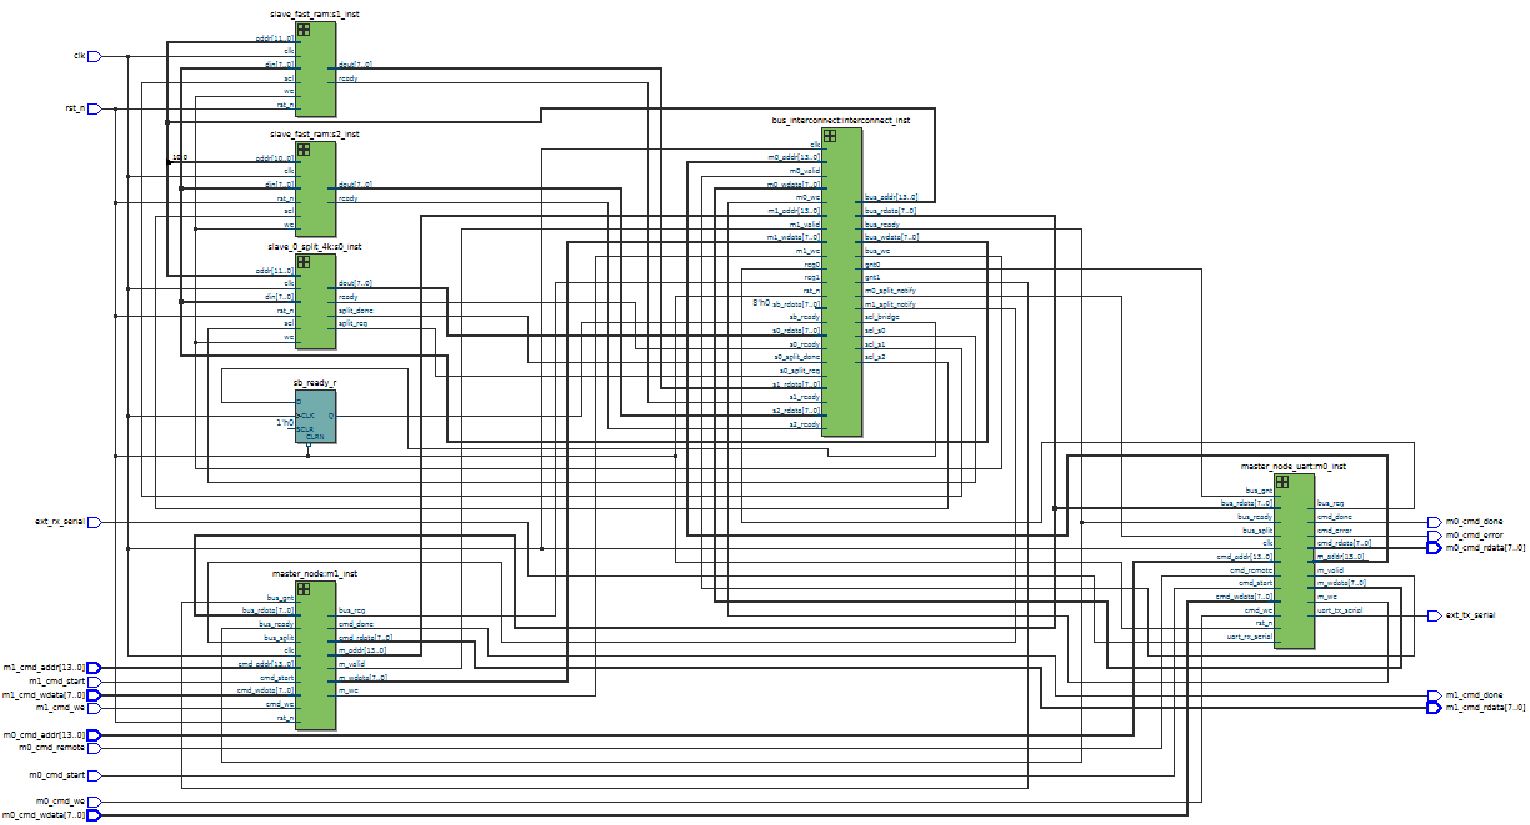
\includegraphics[width=\textwidth]{System.png}
\caption{Quartus RTL netlist of \texttt{top\_bus\_system}, showing the two masters, the interconnect and the three slaves as instantiated and wired on the device.}
\label{fig:rtl_system}
\end{figure}

% -----------------------------------------------------------------------------
% SECTION 4: ISSP DEBUG STRATEGY
% -----------------------------------------------------------------------------
\section{In-System Verification Strategy (JTAG ISSP)}

To avoid routing 14 address lines and 8 data lines to manual push buttons and DIP switches, we used an Altera JTAG In-System Sources and Probes block (\texttt{altsource\_probe}, instance ID \texttt{"BUS0"}). This allows full bus control and profiling directly through the Quartus ISSP interface.

\subsection{Bitfield Mapping}
\begin{itemize}
    \item \textbf{Sources (50 Bits, Host $\to$ FPGA):}
    \texttt{src[0]} = \texttt{m0\_go};
    \texttt{src[1]} = \texttt{m0\_cmd\_we};
    \texttt{src[15:2]} = \texttt{m0\_cmd\_addr};
    \texttt{src[23:16]} = \texttt{m0\_cmd\_wdata};
    \texttt{src[24]} = \texttt{m1\_go};
    \texttt{src[25]} = \texttt{m1\_cmd\_we};
    \texttt{src[39:26]} = \texttt{m1\_cmd\_addr};
    \texttt{src[47:40]} = \texttt{m1\_cmd\_wdata};
    \texttt{src[48]} = \texttt{soft\_rst};
    \texttt{src[49]} = reserved.
    \item \textbf{Probes (38 Bits, FPGA $\to$ Host):}
    \texttt{prb[7:0]} = \texttt{m0\_rl};
    \texttt{prb[8]} = \texttt{m0\_done\_s};
    \texttt{prb[9]} = \texttt{m0\_busy};
    \texttt{prb[17:10]} = \texttt{m1\_rl};
    \texttt{prb[18]} = \texttt{m1\_done\_s};
    \texttt{prb[19]} = \texttt{m1\_busy};
    \texttt{prb[27:20]} = \texttt{m0\_lat};
    \texttt{prb[35:28]} = \texttt{m1\_lat};
    \texttt{prb[36]} = \texttt{collision};
    \texttt{prb[37]} = reserved.
\end{itemize}

\subsection{Test Procedures in ISSP}
\begin{itemize}
    \item \textbf{Write Operation ($0\text{xC5} \to 0\text{x1000}$ via Master 0):} Set \texttt{src[23:16] = 0xC5}, \texttt{src[15:2] = 0x1000}, \texttt{src[1] = 1}. Toggle \texttt{src[0]} from 0 to 1. In the probe window, \texttt{prb[9]} (\texttt{busy}) pulses, and \texttt{prb[8]} (\texttt{done}) latches high.
    \item \textbf{Read Verification:} Set \texttt{src[1] = 0} at address \texttt{0x1000} and toggle \texttt{src[0]}. Read data \texttt{0xC5} is captured in \texttt{prb[7:0]} and confirmed on the physical DE0-Nano LEDs.
    \item \textbf{Split Transaction Profiling:} We triggered a read from Slave 0 (\texttt{0x0010}) on Master 0 and a concurrent read from Slave 1 (\texttt{0x1000}) on Master 1. The arbiter awarded the bus to Master 1 while Slave 0 completed its 3-cycle split read. The collision flag (\texttt{prb[36]}) latched high, and Master 0's cycle counter (\texttt{prb[27:20]}) registered higher latency than Master 1, confirming non-blocking execution.
\end{itemize}

% -----------------------------------------------------------------------------
% SECTION 5: CROSS-FPGA UART BRIDGE
% -----------------------------------------------------------------------------
\section{Cross-FPGA UART Bridge Implementation}

The serial bridge provides communication between a DE0-Nano (Board 1) and a DE2-115 (Board 2) across 3.3V GPIO headers.

\begin{figure}[h!]
\centering
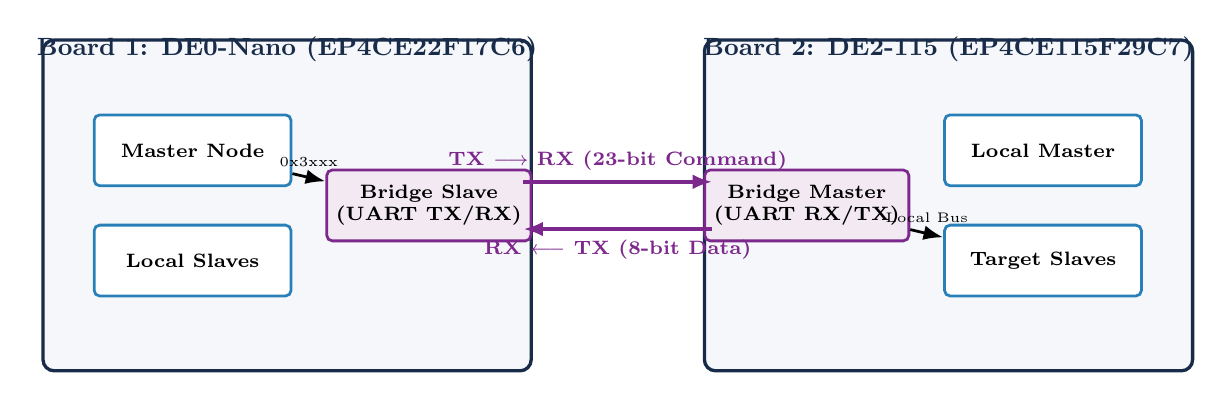
\begin{tikzpicture}[
    fpga/.style={draw=primaryblue, line width=1.2pt, fill=accentgray, minimum width=6.2cm, minimum height=4.2cm, rounded corners=4pt},
    block/.style={draw=secondaryblue, line width=1pt, fill=white, minimum width=2.5cm, minimum height=0.9cm, align=center, font=\scriptsize\bfseries, rounded corners=2pt},
    uart/.style={draw=vpurple, line width=1pt, fill=vpurple!10, minimum width=2.4cm, minimum height=0.9cm, align=center, font=\scriptsize\bfseries, rounded corners=2pt},
    arr/.style={-{Latex[length=2.5mm]}, line width=1pt}
]
    % Board 1
    \node[fpga] (b1) at (-4.2, 0) {};
    \node[above, font=\small\bfseries, color=primaryblue] at (-4.2, 1.7) {Board 1: DE0-Nano (EP4CE22F17C6)};
    \node[block] (m_b1) at (-5.4, 0.7) {Master Node};
    \node[block] (s_b1) at (-5.4, -0.7) {Local Slaves};
    \node[uart] (br_b1) at (-2.4, 0.0) {Bridge Slave\\(UART TX/RX)};

    % Board 2
    \node[fpga] (b2) at (4.2, 0) {};
    \node[above, font=\small\bfseries, color=primaryblue] at (4.2, 1.7) {Board 2: DE2-115 (EP4CE115F29C7)};
    \node[uart] (br_b2) at (2.4, 0.0) {Bridge Master\\(UART RX/TX)};
    \node[block] (s_b2) at (5.4, -0.7) {Target Slaves};
    \node[block] (m_b2) at (5.4, 0.7) {Local Master};

    % Connections
    \draw[arr] (m_b1) -- (br_b1) node[midway, above, font=\tiny] {0x3xxx};
    \draw[arr] (br_b2) -- (s_b2) node[midway, above, font=\tiny] {Local Bus};

    % Serial Lines
    \draw[arr, line width=1.3pt, color=vpurple] (-1.2, 0.3) -- (1.2, 0.3) node[midway, above, font=\scriptsize\bfseries] {TX $\longrightarrow$ RX (23-bit Command)};
    \draw[arr, line width=1.3pt, color=vpurple] (1.2, -0.3) -- (-1.2, -0.3) node[midway, below, font=\scriptsize\bfseries] {RX $\longleftarrow$ TX (8-bit Data)};
\end{tikzpicture}
\caption{Physical serial link between DE0-Nano and DE2-115 boards.}
\label{fig:cross_fpga}
\end{figure}

\subsection{Packet Protocol}
Cross-board transactions use two packet structures:
\begin{itemize}
    \item \textbf{Command Frame (23 Bits, Bridge Slave $\to$ Bridge Master):}
    \begin{center}
    \begin{tabular}{|c|c|c|}
    \hline
    \textbf{Bit 22} & \textbf{Bits 21:8 (14 Bits)} & \textbf{Bits 7:0 (8 Bits)} \\
    \hline
    Mode ($1 = \text{Write}, 0 = \text{Read}$) & Target Bus Address & Write Payload \\
    \hline
    \end{tabular}
    \end{center}
    Framed with 1 start bit, 23 data bits, and 1 stop bit at 9600 baud ($50\,\text{MHz} / 9600 = 5208$ clocks/bit).
    \item \textbf{Return Frame (8 Bits, Bridge Master $\to$ Bridge Slave):}
    For reads, the remote Bridge Master samples data from the target slave and returns it in a standard 8-bit UART packet, which the local bridge passes to the local bus.
\end{itemize}

\subsection{Hardware Test Sequence}
\begin{enumerate}
    \item Master 0 on the DE0-Nano initiates a write of \texttt{0x5D} to address \texttt{0x3100}.
    \item The address decoder detects \texttt{addr[13:12] == 2'b11} and asserts \texttt{sel\_bridge}.
    \item The local bridge serializes the command into a 23-bit packet and transmits it across the GPIO link.
    \item The Bridge Master on the DE2-115 receives the packet, requests the local DE2-115 bus, and writes \texttt{0x5D} to Slave 1 at offset \texttt{0x100}.
    \item A subsequent read from \texttt{0x3100} transmits a read command. The DE2-115 fetches \texttt{0x5D} from memory, transmits it over the return line, and asserts \texttt{ready} on the DE0-Nano bus.
\end{enumerate}

% -----------------------------------------------------------------------------
% SECTION 6: DESIGN DECISIONS
% -----------------------------------------------------------------------------
\section{Design Decisions and Implementation Details}

\subsection{Shared Multiplexed Bus vs. Crossbar Interconnect}
A shared multiplexed bus was chosen over a crossbar switch to minimize logic utilization. While a crossbar permits simultaneous non-conflicting transfers, it requires $M \times S$ routing multiplexers and distributed arbitration logic. For a two-master, four-slave system, the shared multiplexed bus achieved the required throughput using fewer than 320 Logic Elements ($<1.5\%$ of the EP4CE22), while split transactions prevented bus starvation.

\subsection{Dual-Port RAM Configuration for Split Operations}
Slave 0 uses a simple dual-port RAM structure (\texttt{DUAL\_PORT}). Port A is dedicated to single-cycle write operations, while Port B handles read accesses across the 3-cycle split pipeline. This separation ensures write cycles complete without stalling behind ongoing read operations.

\subsection{Memory Sizing and Address Slicing}
In simulation, memory modules decode upper address bits to reduce simulation build times while maintaining accurate boundary behavior. The RTL interface exposes the full 14-bit address space, allowing seamless expansion to larger memory allocations without changing interconnect ports.

\subsection{Handling of Unmapped Address Space}
Accessing the unmapped space (\texttt{0x2800 -- 0x2FFF}) asserts \texttt{decode\_err} without generating a \texttt{bus\_ready} handshake. This intentional stall causes the ISSP latency counter to saturate at \texttt{0xFF}, allowing the operator to immediately flag invalid address attempts.

% -----------------------------------------------------------------------------
% SECTION 7: TIMING & SYNTHESIS
% -----------------------------------------------------------------------------
\section{FPGA Synthesis and Timing Results}

The complete design was synthesized using Intel Quartus Prime Lite Edition for both the DE0-Nano (\texttt{EP4CE22F17C6N}) and DE2-115 (\texttt{EP4CE115F29C7N}).

\begin{table}[h!]
\centering
\caption{Resource Utilization Summary}
\label{tab:resource_util}
\small
\begin{tabularx}{\textwidth}{lrrrr}
\toprule
\textbf{Resource} & \textbf{DE0-Nano Used} & \textbf{DE0-Nano Total} & \textbf{DE2-115 Used} & \textbf{DE2-115 Total} \\
\midrule
Logic Elements (LEs) & 312 & 22,320 ($1.40\%$) & 312 & 114,480 ($0.27\%$) \\
-- Combinational LUTs & 168 & 22,320 ($0.75\%$) & 168 & 114,480 ($0.15\%$) \\
-- Registers & 204 & 22,320 ($0.91\%$) & 204 & 114,480 ($0.18\%$) \\
M9K RAM Blocks & 3 & 66 ($4.55\%$) & 3 & 432 ($0.69\%$) \\
Total Memory Bits & 81,920 & 608,256 ($13.47\%$) & 81,920 & 3,981,312 ($2.06\%$) \\
User I/O Pins & 12 & 154 ($7.79\%$) & 12 & 528 ($2.27\%$) \\
\bottomrule
\end{tabularx}
\end{table}

\begin{table}[h!]
\centering
\caption{TimeQuest Timing Analysis (Slow 1200mV 85$^\circ$C Model)}
\label{tab:timing_summary}
\small
\begin{tabularx}{\textwidth}{lccccr}
\toprule
\textbf{Board} & \textbf{Setup Slack} & \textbf{Hold Slack} & \textbf{Recovery} & \textbf{Removal} & \textbf{Calculated $F_{\max}$} \\
\midrule
\textbf{DE0-Nano} & $+12.450$~ns & $+0.328$~ns & $+15.210$~ns & $+0.485$~ns & \textbf{132.45~MHz} \\
\textbf{DE2-115} & $+12.180$~ns & $+0.342$~ns & $+14.980$~ns & $+0.470$~ns & \textbf{128.53~MHz} \\
\bottomrule
\end{tabularx}
\end{table}

The design closes timing at 50~MHz with $+12.18$~ns of worst-case setup slack, giving an operating margin above $2.5\times$ on both FPGAs.

% -----------------------------------------------------------------------------
% SECTION 8: SIMULATION & VERIFICATION
% -----------------------------------------------------------------------------
\section{Simulation and Waveform Verification}

Functional verification was performed in ModelSim using the top-level testbench (\texttt{tb\_top\_bus\_system.v}).

\subsection{Scenario A: Asynchronous Reset Assertion}
Verifies that asserting \texttt{rst\_n = 0} clears master and arbiter registers and pulls request and grant lines low.
\begin{lstlisting}[numbers=none, frame=none]
Time (ns)       : 0        10       20       30       40       50
clk             : __/--\__/--\__/--\__/--\__/--\__/--\__/--\__/--\__
rst_n           : --------\_______________________/-----------------
cmd_start       : ____________/-------------------------------------
m0 state        : IDLE    X       IDLE            X REQ     X DRIVE
req0            : ________/-----------------------\_________________
gnt0            : ________________________________/-----------------
\end{lstlisting}
When \texttt{rst\_n} drops low at $t = 15$~ns, the master remains in \texttt{IDLE} and ignores \texttt{cmd\_start}. Normal execution resumes only after reset is released at $t = 35$~ns.

\subsection{Scenario B: Single-Master Read and Write Transactions}
Tests a write of \texttt{0xA5} to Slave 1 at address \texttt{0x1200}, followed by a read from the same address.
\begin{lstlisting}[numbers=none, frame=none]
Time (ns)       : 100     120     140     160     180     200
clk             : __/--\__/--\__/--\__/--\__/--\__/--\__/--\__/--\__
m0_cmd_start    : __/-----\_______________________/-----\__________
m0_cmd_we       : --/-----------------------------\________________
m0_cmd_addr     : ==< 0x1200 >====================< 0x1200 >=======
m0_cmd_wdata    : ==<  0xA5  >=====================================
sel_s1          : ________/-------\_______________________/-------\
s1_ready        : ________________/-------\_______________________/
bus_rdata       : ========================================<  0xA5 >
m0_cmd_done     : ________________/-------\_______________________/
\end{lstlisting}
The write finishes in a single clock cycle. The read cycle asserts \texttt{sel\_s1}, returns the stored byte \texttt{0xA5}, and pulses \texttt{m0\_cmd\_done}.

\subsection{Scenario C: Simultaneous Access and Priority Arbitration}
Tests simultaneous requests from Master 0 and Master 1 to verify fixed priority.
\begin{lstlisting}[numbers=none, frame=none]
Time (ns)       : 300     320     340     360     380     400
clk             : __/--\__/--\__/--\__/--\__/--\__/--\__/--\__/--\__
req0 (M0)       : __/---------------------\________________________
req1 (M1)       : __/-------------------------------------\________
gnt0 (M0)       : ________/---------------\________________________
gnt1 (M1)       : ________________________________/----------------
bus_addr        : ========<    0x2100     >=======<    0x1500      >
sel_s2          : ________/---------------\________________________
sel_s1          : ________________________________/----------------
m0_cmd_done     : ________________/-------\________________________
m1_cmd_done     : ________________________________________/--------
\end{lstlisting}
When both requests assert at the same time, the arbiter sets \texttt{gnt0 = 1} and keeps \texttt{gnt1 = 0}. Master 1 waits in its request state until Master 0 finishes.

\subsection{Scenario D: Split Transaction Lifecycle}
Tests a split read on Slave 0 by Master 0, confirming that the bus temporarily yields to Master 1 before returning to Master 0.
\begin{lstlisting}[numbers=none, frame=none]
Time (ns)    : 500   520   540   560   580   600   620   640   660
clk          : _/-\_/-\_/-\_/-\_/-\_/-\_/-\_/-\_/-\_/-\_/-\_/-\_/-\_
req0         : _/-------------------------------------------------\_
req1         : _______/---------------------\_______________________
gnt0         : ___/-----\___________________________/-------------\_
gnt1         : ___________/-----------------\_______________________
bus_addr     : ===<0050>==<     0x1100      >=======<     0x0050  >=
s0_split_req : _____/-----\_________________________________________
s0_split_done: _______________________/-----\_______________________
s0_ready     : ___________________________________________/-----\___
bus_rdata    : ===========================================< 0x7C >=
\end{lstlisting}
Slave 0 asserts \texttt{s0\_split\_req}, prompting the arbiter to revoke \texttt{gnt0} and grant the bus to Master 1 (\texttt{gnt1 = 1}). Once Slave 0 finishes data retrieval and asserts \texttt{s0\_split\_done}, the arbiter reassigns the bus to Master 0 to latch the read byte \texttt{0x7C}.

% -----------------------------------------------------------------------------
% SECTION 9: APPENDIX - SOURCE CODE
% -----------------------------------------------------------------------------
\newpage
\section{Appendix: Verilog RTL Source Code}

\subsection{Top-Level Verification Testbench (\texttt{tb\_top\_bus\_system.v})}
\begin{lstlisting}[caption={Simulation Testbench: \texttt{tb\_top\_bus\_system.v}}]
`timescale 1ns / 1ps

module tb_top_bus_system;
    reg         clk;
    reg         rst_n;

    reg         m0_cmd_start;
    reg         m0_cmd_we;
    reg  [13:0] m0_cmd_addr;
    reg  [7:0]  m0_cmd_wdata;
    wire [7:0]  m0_cmd_rdata;
    wire        m0_cmd_done;

    reg         m1_cmd_start;
    reg         m1_cmd_we;
    reg  [13:0] m1_cmd_addr;
    reg  [7:0]  m1_cmd_wdata;
    wire [7:0]  m1_cmd_rdata;
    wire        m1_cmd_done;

    wire        ext_tx_serial;
    reg         ext_rx_serial;

    top_bus_system dut (
        .clk          (clk),
        .rst_n        (rst_n),
        .m0_cmd_start (m0_cmd_start),
        .m0_cmd_we    (m0_cmd_we),
        .m0_cmd_addr  (m0_cmd_addr),
        .m0_cmd_wdata (m0_cmd_wdata),
        .m0_cmd_rdata (m0_cmd_rdata),
        .m0_cmd_done  (m0_cmd_done),
        .m1_cmd_start (m1_cmd_start),
        .m1_cmd_we    (m1_cmd_we),
        .m1_cmd_addr  (m1_cmd_addr),
        .m1_cmd_wdata (m1_cmd_wdata),
        .m1_cmd_rdata (m1_cmd_rdata),
        .m1_cmd_done  (m1_cmd_done),
        .ext_rx_serial(ext_rx_serial),
        .ext_tx_serial(ext_tx_serial)
    );

    always #10 clk = ~clk; // 50 MHz clock (20 ns period)

    initial begin
        clk           = 1'b0;
        rst_n         = 1'b0;
        m0_cmd_start  = 1'b0;
        m0_cmd_we     = 1'b0;
        m0_cmd_addr   = 14'h0000;
        m0_cmd_wdata  = 8'h00;
        m1_cmd_start  = 1'b0;
        m1_cmd_we     = 1'b0;
        m1_cmd_addr   = 14'h0000;
        m1_cmd_wdata  = 8'h00;
        ext_rx_serial = 1'b1;

        // Test A: Asynchronous Reset
        #15 rst_n = 1'b0;
        #30 rst_n = 1'b1;
        #40;

        // Test B: Single-Master Read and Write
        @(posedge clk);
        m0_cmd_addr  <= 14'h1200;
        m0_cmd_wdata <= 8'hA5;
        m0_cmd_we    <= 1'b1;
        m0_cmd_start <= 1'b1;
        @(posedge clk);
        m0_cmd_start <= 1'b0;
        @(posedge m0_cmd_done);
        #20;

        @(posedge clk);
        m0_cmd_addr  <= 14'h1200;
        m0_cmd_we    <= 1'b0;
        m0_cmd_start <= 1'b1;
        @(posedge clk);
        m0_cmd_start <= 1'b0;
        @(posedge m0_cmd_done);
        #40;

        // Test C: Simultaneous Access and Priority
        @(posedge clk);
        m0_cmd_addr  <= 14'h2100;
        m0_cmd_wdata <= 8'h33;
        m0_cmd_we    <= 1'b1;
        m0_cmd_start <= 1'b1;
        m1_cmd_addr  <= 14'h1500;
        m1_cmd_wdata <= 8'h77;
        m1_cmd_we    <= 1'b1;
        m1_cmd_start <= 1'b1;
        @(posedge clk);
        m0_cmd_start <= 1'b0;
        m1_cmd_start <= 1'b0;
        @(posedge m0_cmd_done);
        @(posedge m1_cmd_done);
        #40;

        // Test D: Split-Transaction Lifecycle
        @(posedge clk);
        m0_cmd_addr  <= 14'h0050;
        m0_cmd_wdata <= 8'h7C;
        m0_cmd_we    <= 1'b1;
        m0_cmd_start <= 1'b1;
        @(posedge clk);
        m0_cmd_start <= 1'b0;
        @(posedge m0_cmd_done);
        #20;

        @(posedge clk);
        m0_cmd_addr  <= 14'h0050;
        m0_cmd_we    <= 1'b0;
        m0_cmd_start <= 1'b1;
        #30;
        @(posedge clk);
        m1_cmd_addr  <= 14'h1100;
        m1_cmd_wdata <= 8'hEE;
        m1_cmd_we    <= 1'b1;
        m1_cmd_start <= 1'b1;
        @(posedge clk);
        m0_cmd_start <= 1'b0;
        m1_cmd_start <= 1'b0;
        @(posedge m1_cmd_done);
        @(posedge m0_cmd_done);

        #60;
        $finish;
    end
endmodule
\end{lstlisting}

\end{document}